\documentclass[aspectratio=169]{beamer}
\usetheme{CambridgeUS}
\usecolortheme{whale}
\useinnertheme{circles}
\useoutertheme{infolines}

% Adjust margins and spacing
\setbeamersize{text margin left=1cm,text margin right=1cm}

% Enhanced frame title template
\setbeamertemplate{frametitle}{%
  \nointerlineskip%
  \begin{beamercolorbox}[wd=\paperwidth,ht=2.5ex,dp=1.125ex]{frametitle}%
    \hspace*{2ex}\insertframetitle%
  \end{beamercolorbox}%
}

% Make frame titles more prominent
\setbeamerfont{frametitle}{size=\large,series=\bfseries}
\setbeamercolor{frametitle}{fg=white,bg=ftmblue}

% Reduce vertical spacing between items globally
\setlength{\itemsep}{0.15ex}
\setlength{\parskip}{0.15ex}

% Adjust frame margins and navigation
\setbeamertemplate{navigation symbols}{}

% Adjust block spacing
\setbeamertemplate{blocks}[rounded][shadow=true]
\addtobeamertemplate{block begin}{\vspace{0.0cm}}{\vspace{0.1cm}}
\addtobeamertemplate{block alerted begin}{\vspace{0.0cm}}{\vspace{0.1cm}}
\addtobeamertemplate{itemize/enumerate body begin}{\vspace{0.13cm}}{}
\addtobeamertemplate{itemize/enumerate item}{\vspace{0.1cm}}{}

% Adjust column spacing
\setlength{\columnsep}{0.5cm}

% Adjust frame content vertical spacing
\addtobeamertemplate{frame begin}{\vspace{0.1cm}}{}
\addtobeamertemplate{frame end}{\vspace{0.1cm}}{}

% Define colors
\definecolor{ftmblue}{RGB}{0, 83, 159}
\definecolor{ftmgreen}{RGB}{0, 128, 128}

% Set theme colors
\setbeamercolor{structure}{fg=ftmblue}
\setbeamercolor{title}{fg=white,bg=ftmblue}
\setbeamercolor{titlelike}{fg=white,bg=ftmblue}
\setbeamercolor{subtitle}{fg=white,bg=ftmblue}
\setbeamercolor{frametitle}{fg=white,bg=ftmblue}
\setbeamercolor{section in head/foot}{fg=white,bg=ftmblue}

% Make titles more prominent
\setbeamerfont{title}{size=\Large,series=\bfseries}
\setbeamerfont{subtitle}{size=\large}
\setbeamerfont{frametitle}{size=\large,series=\bfseries}

\usepackage{graphicx}
\usepackage{booktabs}
\usepackage{fontawesome5}
\usepackage{tikz}
\usepackage{multicol}
\usetikzlibrary{mindmap,trees,shadows}

% Custom command for placeholder images - adjusted height
\newcommand{\placeholderimage}[1]{%
    \begin{center}
        \fbox{\begin{minipage}[c][0.4\textheight][c]{0.8\textwidth}
            \centering\large #1
        \end{minipage}}
    \end{center}%
}

\title{FTM/JJ Private Hospital\\AI-Powered EHR Implementation Project}
\subtitle{Transforming Healthcare Delivery through Intelligent Systems}
\author{ICT Management Team}
\date{\today}
\logo{\includegraphics[width=2.0cm]{SKTedtech_360.png}}

% Customize TOC appearance
\setbeamertemplate{section in toc}[sections numbered]
\setbeamercolor{section in toc}{fg=black}
\setbeamercolor{section in toc shaded}{fg=gray}
\setbeamertemplate{section in toc shaded}[default][50]

% Remove the automatic section pages
\AtBeginSection[]{}

\begin{document}

%----------------------------------------------------------
% Title slide
%----------------------------------------------------------
\begin{frame}
    \titlepage
\end{frame}

%----------------------------------------------------------
% Table of Contents (two-column version)
%----------------------------------------------------------
\begin{frame}{Table of Contents}
    \begin{multicols}{2}
        \small
        \tableofcontents[hideallsubsections]
    \end{multicols}
\end{frame}

%----------------------------------------------------------
% Introduction
%----------------------------------------------------------
\section{Project Overview}
\begin{frame}{Project Overview}
    \begin{columns}[T]
        \column{1.0\textwidth}
        \begin{center}
            \includegraphics[height=0.8\textheight]{title_illustration.png}
            %\vspace{0.2cm}
        \end{center}
    \end{columns}
\end{frame}

%----------------------------------------------------------
% Current Challenges
%----------------------------------------------------------
\section{Current Challenges}
\begin{frame}{Current Challenges}
    \begin{columns}[T]
        \column{1.0\textwidth}
        \begin{center}
            \includegraphics[height=0.8\textheight]{problem_illustration.png}
        \end{center}
    \end{columns}
\end{frame}

%----------------------------------------------------------
% System Overview
%----------------------------------------------------------
\section{System Overview}
\begin{frame}{System Overview}
    \begin{columns}[T]
        \column{1.0\textwidth}
        \begin{center}
            \includegraphics[height=0.8\textheight]{outline_illustration.png}
        \end{center}
    \end{columns}
\end{frame}

%----------------------------------------------------------
% The Opportunity
%----------------------------------------------------------
\section{The Opportunity}
\begin{frame}{The Opportunity}
    \begin{columns}[T]
        \column{0.5\textwidth}
            \begin{block}{Current Challenges}
                \begin{itemize}
                    \item Fragmented patient records
                    \item Limited healthcare access
                    \item Manual process inefficiencies
                    \item Security vulnerabilities
                \end{itemize}
            \end{block}
            
            \begin{alertblock}{The Opportunity}
                Implement an AI-powered EHR system to transform healthcare delivery in underserved regions
            \end{alertblock}
        \column{0.5\textwidth}
            \includegraphics[width=0.8\textwidth]{intro_illustration.png}
    \end{columns}
\end{frame}

%----------------------------------------------------------
% Problem Statement
%----------------------------------------------------------
\section{Problem Statement}
\begin{frame}{Problem Statement}
    \begin{columns}[T]
        \column{0.5\textwidth}
            \begin{quote}
                \large In remote African regions, private hospitals face challenges in care delivery. The lack of a centralized system leads to inefficiencies and compromised care. This project presents an opportunity to implement an AI-powered EHR system that improves clinical workflows and efficiency.
            \end{quote}
            

        \column{0.5\textwidth}
            \includegraphics[width=0.7\textwidth]{problem_illustration.png}
    \end{columns}
    \vspace{0.1cm}
    
\begin{tikzpicture}
        \node[draw=ftmblue, rounded corners, fill=blue!10, text width=\textwidth, align=center] {
            Transforming healthcare through intelligent systems and patient-centric design
        };
    \end{tikzpicture}
\end{frame}

%----------------------------------------------------------
% Top Features
%----------------------------------------------------------
\section{Key Features of AI-Powered EHR}
\begin{frame}{Key Features of AI-Powered EHR}
    \begin{columns}[T]
        \column{0.5\textwidth}
            \begin{enumerate}
                \item \textbf{Secure Patient Registration}\\
                Biometric verification, digital profiles
                
                \item \textbf{Patient Self-Service Portal}\\
                Mobile app for records, appointments
                
                \item \textbf{AI Clinical Decision Support}\\
                Diagnosis assistance, treatment planning
                
                \item \textbf{Integrated Payment System}\\
                Digital transactions, receipts
                
                \item \textbf{Analytics Dashboard}\\
                Trends, resource utilization
            \end{enumerate}
        \column{0.5\textwidth}
            \includegraphics[width=0.8\textwidth]{features_illustration.png}
    \end{columns}
\end{frame}

%----------------------------------------------------------
% Feature Spotlight: Patient Self-Service
%----------------------------------------------------------
\section{Patient Self-Service Portal}
\begin{frame}{Patient Self-Service Portal}
    \begin{columns}[T]
        \column{0.5\textwidth}
            \begin{block}{Key Capabilities}
                \begin{itemize}
                    \item \faIcon{calendar-alt}\ Schedule appointments
                    \item \faIcon{file-alt}\ Access medical records
                    \item \faIcon{pills}\ Medication reminders
                    \item \faIcon{credit-card}\ Bill payments
                \end{itemize}
            \end{block}
            
            \begin{alertblock}{Patient Benefits}
                \begin{itemize}
                    \item Reduced waiting times
                    \item Greater care engagement
                    \item Enhanced communication
                \end{itemize}
            \end{alertblock}
        \column{0.5\textwidth}
            \includegraphics[width=0.8\textwidth]{patient_portal_illustration.png}
    \end{columns}
\end{frame}

%----------------------------------------------------------
% Feature Spotlight: AI Clinical Decision Support
%----------------------------------------------------------
\section{AI Clinical Decision Support}
\begin{frame}{AI Clinical Decision Support}
    \begin{columns}[T]
        \column{0.5\textwidth}
            \begin{block}{Clinical Intelligence}
                \begin{itemize}
                    \item Pattern recognition in patient data
                    \item Evidence-based treatment suggestions
                    \item Risk stratification tools
                    \item Treatment outcome predictions
                \end{itemize}
            \end{block}
            
            \begin{alertblock}{Healthcare Provider Benefits}
                \begin{itemize}
                    \item Enhanced diagnostic accuracy
                    \item Reduced medical errors
                    \item Standardized care protocols
                \end{itemize}
            \end{alertblock}
        \column{0.5\textwidth}
            \includegraphics[width=0.8\textwidth]{ai_clinical_illustration.png}
    \end{columns}
\end{frame}

%----------------------------------------------------------
% Success Criteria
%----------------------------------------------------------
\section{Project Success Criteria}
\begin{frame}{Project Success Criteria}
    \begin{columns}[T]
        \column{0.55\textwidth}
            \begin{center}
                \begin{tabular}{lc}
                    \toprule
                    \textbf{Key Performance Indicator} & \textbf{Target} \\
                    \midrule
                    System Adoption Rate & 85\% \\
                    Patient Waiting Time Reduction & 40\% \\
                    Data Security Compliance & 100\% \\
                    Clinical Decision Accuracy & +25\% \\
                    Digital Payment Success & 90\%+ \\
                    \bottomrule
                \end{tabular}
            \end{center}
        \column{0.45\textwidth}
            \hspace{0.5cm}\includegraphics[width=0.8\textwidth]{kpi_illustration.png}
    \end{columns}
\end{frame}

%----------------------------------------------------------
% Implementation Timeline
%----------------------------------------------------------
\section{Implementation Timeline}
\begin{frame}{Implementation Timeline}
    \begin{columns}[T]
        \column{0.1\textwidth}
            \begin{center}
                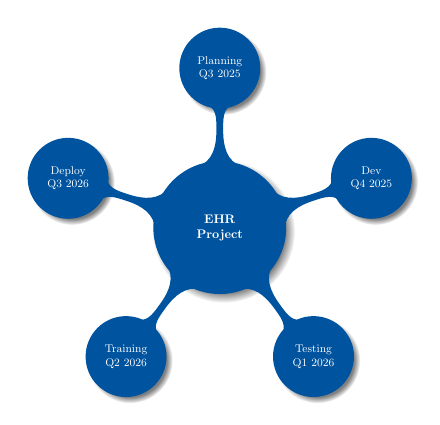
\begin{tikzpicture}[
                    mindmap,
                    concept color=ftmblue,
                    text=white,
                    scale=0.45,
                    transform shape,
                    every node/.style={
                        concept,
                        circular drop shadow,
                        execute at begin node=\hspace{0pt},
                        font=\small
                    },
                    root concept/.append style={
                        concept color=ftmblue,
                        font=\normalsize\bfseries,
                        minimum size=1.6cm
                    },
                    level 1/.append style={
                        font=\small,
                        sibling angle=72,
                        level distance=4.5cm,
                        minimum size=1.4cm
                    }
                ]
                    \node[root concept] {EHR\\Project}
                    [clockwise from=90]
                        child { node[concept] {Planning\\Q3 2025} }
                        child { node[concept] {Dev\\Q4 2025} }
                        child { node[concept] {Testing\\Q1 2026} }
                        child { node[concept] {Training\\Q2 2026} }
                        child { node[concept] {Deploy\\Q3 2026} };
                \end{tikzpicture}
            \end{center}
            
            \vspace{0.2cm}

        \column{0.9\textwidth}
        \begin{description}[leftmargin=0em,itemsep=0.2ex]
            \item[Q3 2025] Requirements finalization, vendor selection
            \item[Q4 2025] System development and customization
            \item[Q1 2026] Testing, user acceptance, and refinement
            \item[Q2 2026] Staff training and patient education
            \item[Q3 2026] Full system deployment and go-live
        \end{description}
        
    \end{columns}
\end{frame}

\begin{frame}{Implementation Timeline}
    \includegraphics[height=0.9\textheight]{roadmap_illustration.png}
\end{frame}

%----------------------------------------------------------
% Expected Benefits
%----------------------------------------------------------
\section{Expected Benefits}
\begin{frame}{Expected Benefits}
    \begin{columns}[T]
        \column{0.5\textwidth}
            \begin{block}{For Patients}
                \begin{itemize}
                    \item Improved care quality
                    \item Enhanced access to services
                    \item Better communication
                \end{itemize}
            \end{block}
            
            \begin{block}{For Healthcare Providers}
                \begin{itemize}
                    \item Accurate clinical decisions
                    \item Reduced admin burden
                    \item Evidence-based support
                \end{itemize}
            \end{block}
            

        \column{0.5\textwidth}
            \begin{block}{For FTM/JJ Hospital}
                \begin{itemize}
                    \item Improved efficiency
                    \item Enhanced revenue management
                    \item Data-driven decisions
                \end{itemize}
            \end{block}
    \end{columns}
\end{frame}

%----------------------------------------------------------
% Next Steps
%----------------------------------------------------------
\section{Next Steps}
\begin{frame}{Next Steps}
    \begin{columns}[T]
        \column{0.4\textwidth}
            \begin{block}{Key Takeaways}
                \begin{itemize}
                    \item Strategic investment in AI-EHR
                    \item Addresses core challenges
                    \item Patient-centered design
                \end{itemize}
            \end{block}
            
            \begin{alertblock}{Next Steps}
                \begin{enumerate}
                    \item Secure executive sponsorship
                    \item Finalize requirements
                    \item Form implementation team
                \end{enumerate}
            \end{alertblock}
            

        \column{0.6\textwidth}
            \begin{center}
                \includegraphics[height=0.6\textheight]{conclusion_illustration.png}
                \vspace{0.2cm}
                \begin{tabular}{lc}
                    \faIcon{envelope} & ict@ftmhospital.org \\[0.2cm]
                    \faIcon{phone} & +123 456 7890 \\
                \end{tabular}
            \end{center}
    \end{columns}
\end{frame}

\end{document}
